% =========================================================
% Stern--Brocot Tree with Sentinels
% =========================================================

\begin{figure}[h]
\centering
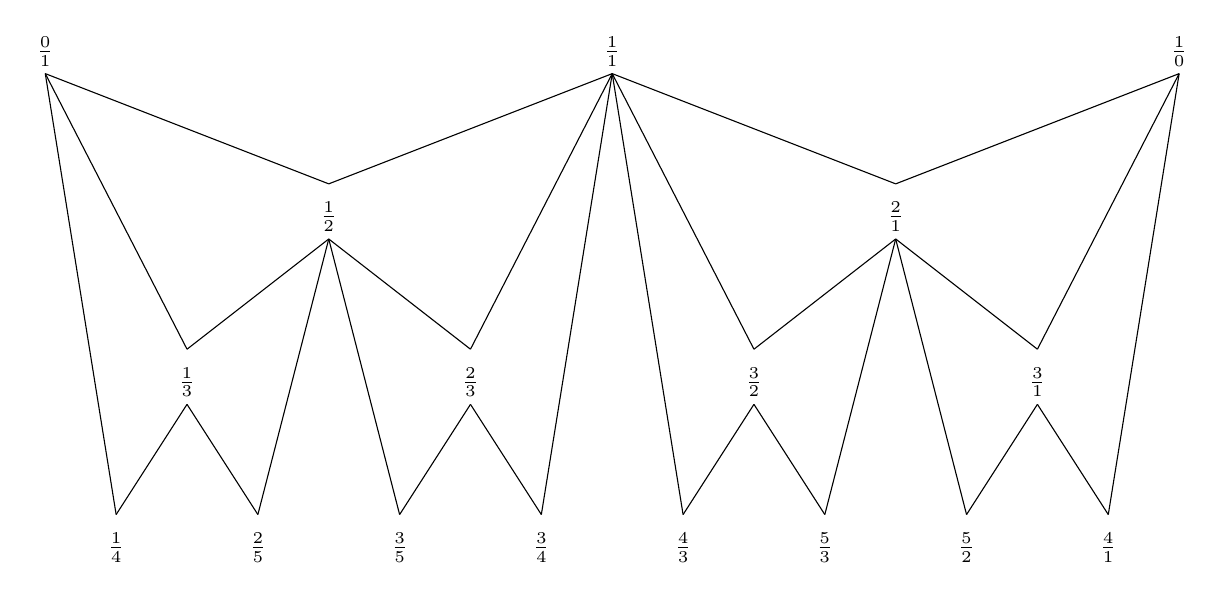
\begin{tikzpicture}[x=1.2cm,y=1.4cm, every node/.style={font=\small}]

% Top sentinels and root
\node at (-6,0) {$\frac{0}{1}$};
\node at ( 0,0) {$\frac{1}{1}$};
\node at ( 6,0) {$\frac{1}{0}$};

% Level 1
\node at (-3,-1.5) {$\frac{1}{2}$};
\node at ( 3,-1.5) {$\frac{2}{1}$};

% Level 2
\node at (-4.5,-3) {$\frac{1}{3}$};
\node at (-1.5,-3) {$\frac{2}{3}$};
\node at ( 1.5,-3) {$\frac{3}{2}$};
\node at ( 4.5,-3) {$\frac{3}{1}$};

% Level 3
\node at (-5.25,-4.5) {$\frac{1}{4}$};
\node at (-3.75,-4.5) {$\frac{2}{5}$};
\node at (-2.25,-4.5) {$\frac{3}{5}$};
\node at (-0.75,-4.5) {$\frac{3}{4}$};
\node at ( 0.75,-4.5) {$\frac{4}{3}$};
\node at ( 2.25,-4.5) {$\frac{5}{3}$};
\node at ( 3.75,-4.5) {$\frac{5}{2}$};
\node at ( 5.25,-4.5) {$\frac{4}{1}$};

% Edges from root to sentinels
\draw (-6,-0.2) -- (-3,-1.2);
\draw ( 0,-0.2) -- (-3,-1.2);
\draw ( 0,-0.2) -- ( 3,-1.2);
\draw ( 6,-0.2) -- ( 3,-1.2);

% Edges level 1 to level 2
\draw (-6,-0.2) -- (-4.5,-2.7);
\draw (-3,-1.7) -- (-4.5,-2.7);
\draw (-3,-1.7) -- (-1.5,-2.7);
\draw ( 0,-0.2) -- (-1.5,-2.7);
\draw ( 0,-0.2) -- ( 1.5,-2.7);
\draw ( 3,-1.7) -- ( 1.5,-2.7);
\draw ( 3,-1.7) -- ( 4.5,-2.7);
\draw ( 6,-0.2) -- ( 4.5,-2.7);

% Edges level 2 to level 3
\draw (-6,-0.2) -- (-5.25,-4.2);
\draw (-4.5,-3.2) -- (-5.25,-4.2);
\draw (-4.5,-3.2) -- (-3.75,-4.2);
\draw (-3,-1.7)   -- (-3.75,-4.2);
\draw (-3,-1.7)   -- (-2.25,-4.2);
\draw (-1.5,-3.2) -- (-2.25,-4.2);
\draw (-1.5,-3.2) -- (-0.75,-4.2);
\draw ( 0,-0.2)   -- (-0.75,-4.2);
\draw ( 0,-0.2)   -- ( 0.75,-4.2);
\draw ( 1.5,-3.2) -- ( 0.75,-4.2);
\draw ( 1.5,-3.2) -- ( 2.25,-4.2);
\draw ( 3,-1.7)   -- ( 2.25,-4.2);
\draw ( 3,-1.7)   -- ( 3.75,-4.2);
\draw ( 4.5,-3.2) -- ( 3.75,-4.2);
\draw ( 4.5,-3.2) -- ( 5.25,-4.2);
\draw ( 6,-0.2)   -- ( 5.25,-4.2);

\end{tikzpicture}
\caption{The Stern--Brocot tree with sentinel fractions $0/1$ and $1/0$.  Each new fraction is the
mediant of its two parent bounds.  Every positive rational number appears exactly once in reduced
form.}
\label{fig:stern-brocot-tree}
\end{figure}


\FloatBarrier
